
\documentclass[border=10pt, 12pt]{standalone}
\usepackage[svgnames]{xcolor}
\usepackage{amsmath}
\usepackage{pgfplots}
\pgfplotsset{compat=newest}
\usepackage[sfdefault]{FiraSans}
\usepackage{FiraMono}
\renewcommand*\familydefault{\sfdefault}
\begin{document}
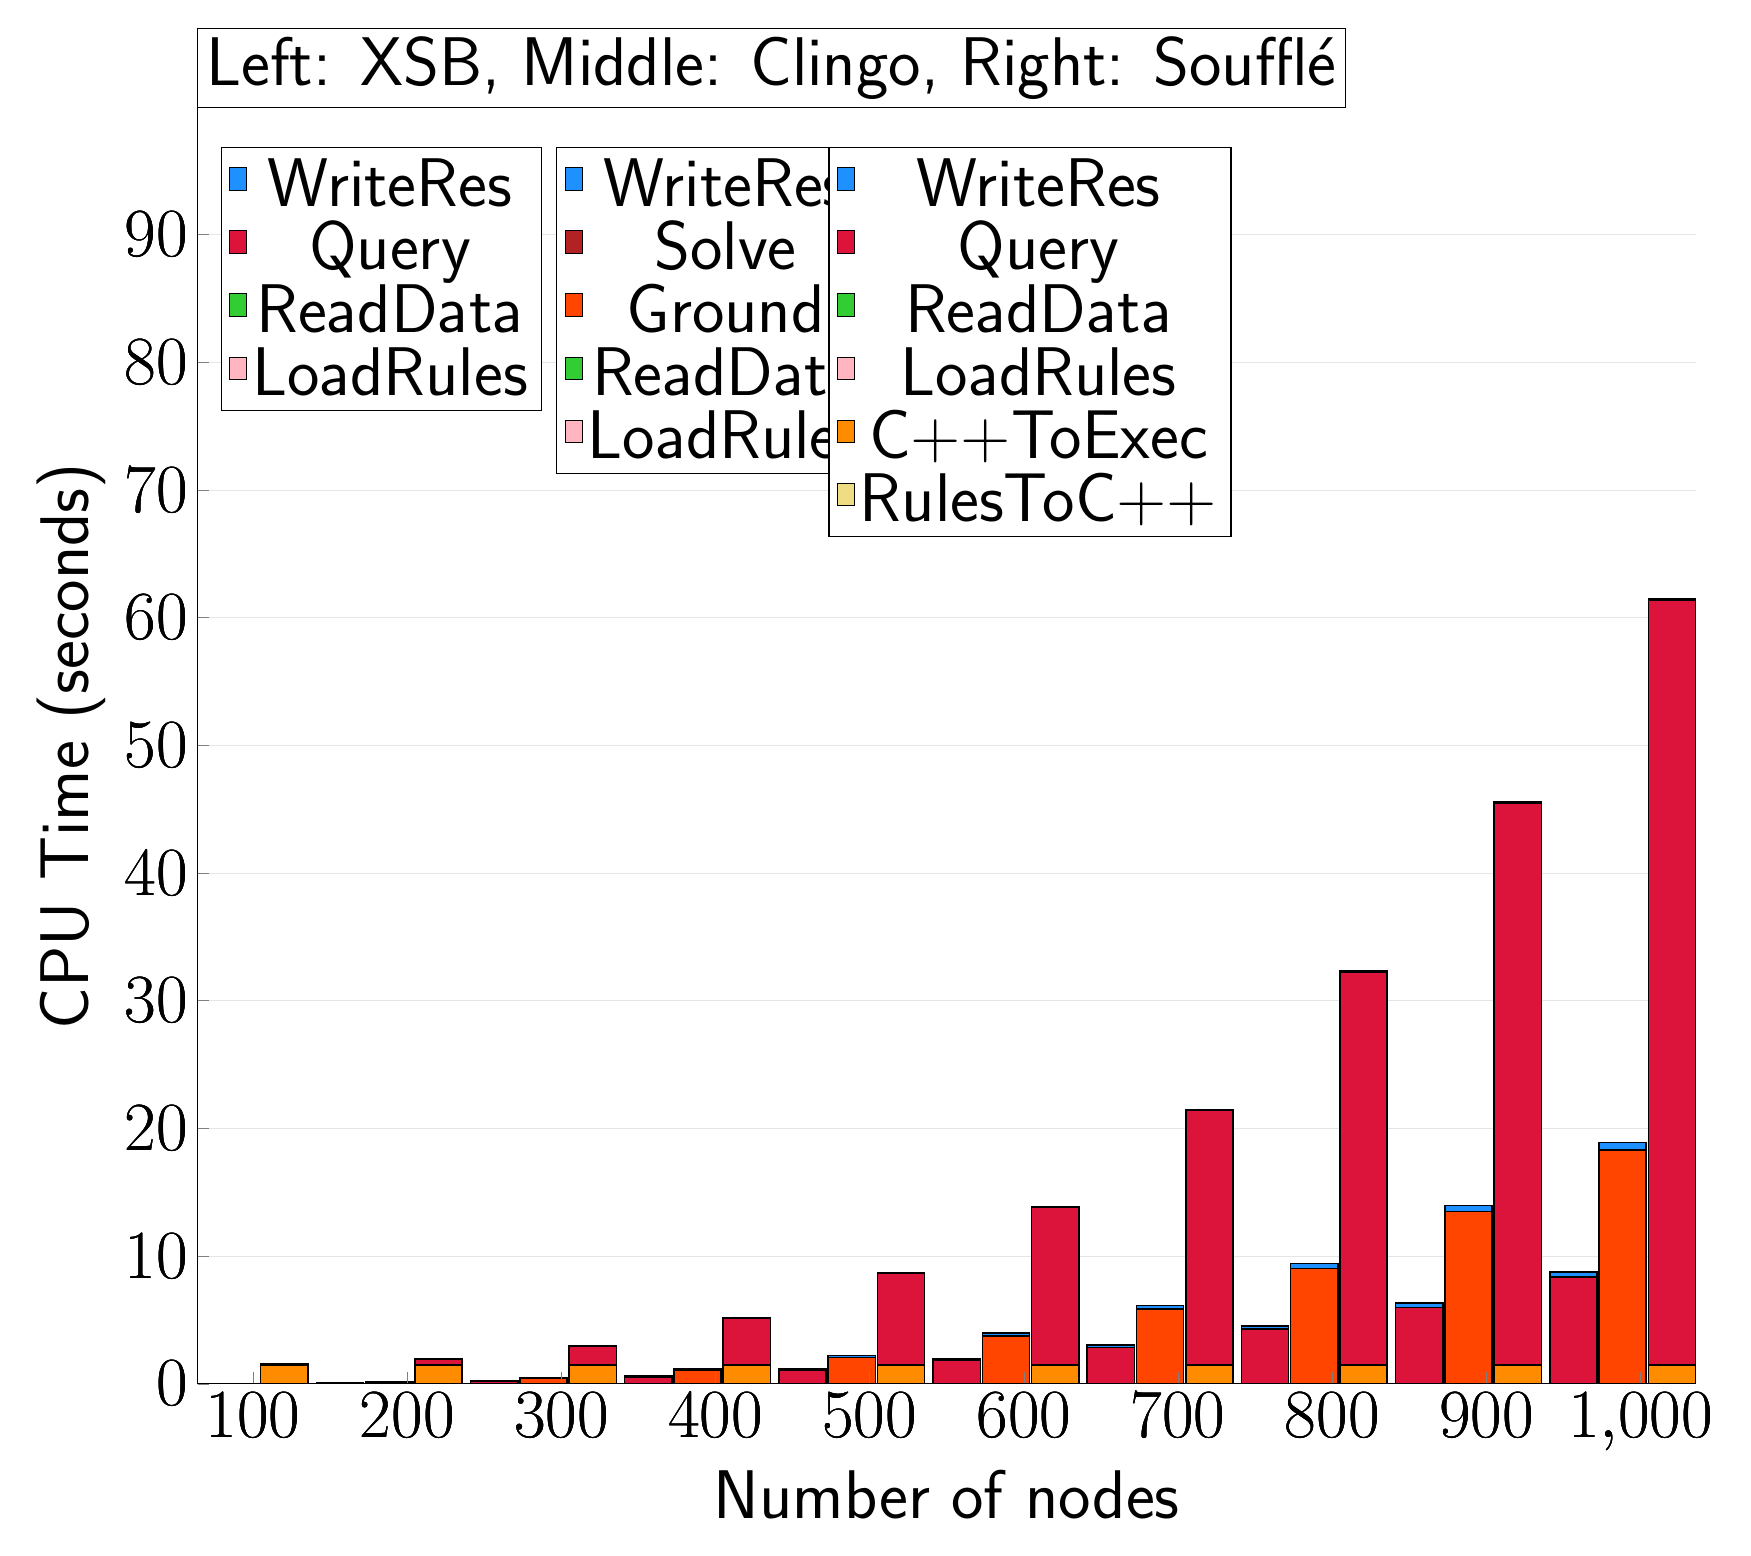
\begin{tikzpicture}
                        \begin{axis}[bar shift=-24.3pt, 
   ybar stacked,
   width=1.7\textwidth,
   bar width=0.6cm,
   ymajorgrids, tick align=inside,
   major grid style={draw=gray!20},
   xtick=data,
   ymin=0, ymax=99.8926,
   axis x line*=bottom,
   axis y line*=left,
   enlarge x limits=0.04,
   legend style={
       at={(0.23, 0.97)},
       anchor=north east,
       legend columns=1,
       font=\Huge,
   },
   ylabel={CPU Time (seconds)},
   xlabel={Number of nodes},
   label style={font=\Huge},
   tick label style={font=\Huge},
]
\addlegendimage{fill=DodgerBlue, draw=black, line width=0.2pt}
\addlegendentry{WriteRes}
\addlegendimage{fill=Crimson, draw=black, line width=0.2pt}
\addlegendentry{Query}
\addlegendimage{fill=LimeGreen, draw=black, line width=0.2pt}
\addlegendentry{ReadData}
\addlegendimage{fill=LightPink, draw=black, line width=0.2pt}
\addlegendentry{LoadRules}
\addplot +[fill=LightPink, draw=black, line width=0.55pt] coordinates {
(100, 0.0005510000000000001)
(200, 0.0005468)
(300, 0.0005496000000000003)
(400, 0.0005499999999999999)
(500, 0.0005500000000000002)
(600, 0.0005492000000000002)
(700, 0.0005675999999999999)
(800, 0.0005501999999999997)
(900, 0.0005510000000000008)
(1000, 0.0005514000000000002)
};
\addplot +[fill=LimeGreen, draw=black, line width=0.55pt] coordinates {
(100, 0.00019679999999999963)
(200, 0.0002732000000000002)
(300, 0.0003530000000000002)
(400, 0.00043459999999999983)
(500, 0.0005156000000000008)
(600, 0.0005881999999999996)
(700, 0.0006672000000000003)
(800, 0.0007433999999999995)
(900, 0.0008229999999999993)
(1000, 0.0009037999999999995)
};
\addplot +[fill=Crimson, draw=black, line width=0.55pt] coordinates {
(100, 0.008066799999999999)
(200, 0.06690700000000001)
(300, 0.22339959999999998)
(400, 0.5394274)
(500, 1.0607646000000002)
(600, 1.810701)
(700, 2.8402032000000004)
(800, 4.2834094)
(900, 5.9626014)
(1000, 8.344221600000001)
};
\addplot +[fill=DodgerBlue, draw=black, line width=0.55pt] coordinates {
(100, 0.0041798)
(200, 0.016567199999999997)
(300, 0.03844740000000001)
(400, 0.06405619999999998)
(500, 0.1006624)
(600, 0.1456886)
(700, 0.20434100000000005)
(800, 0.24269459999999993)
(900, 0.35166140000000007)
(1000, 0.4282771999999998)
};
\end{axis}

\begin{axis}[bar shift=-6.5pt, 
   ybar stacked,
   width=1.7\textwidth,
   bar width=0.6cm,
   ymajorgrids, tick align=inside,
   major grid style={draw=none},
   xtick=data,
   ymin=0, ymax=99.8926,
   axis x line*=none,
   axis y line*=none,
   enlarge x limits=0.04,
   legend style={
       at={(0.454, 0.97)},
       anchor=north east,
       legend columns=1,
       font=\Huge,
   },
   label style={font=\Huge},
   tick label style={font=\Huge},
]
\addlegendimage{fill=DodgerBlue, draw=black, line width=0.2pt}
\addlegendentry{WriteRes}
\addlegendimage{fill=FireBrick, draw=black, line width=0.2pt}
\addlegendentry{Solve}
\addlegendimage{fill=OrangeRed, draw=black, line width=0.2pt}
\addlegendentry{Ground}
\addlegendimage{fill=LimeGreen, draw=black, line width=0.2pt}
\addlegendentry{ReadData}
\addlegendimage{fill=LightPink, draw=black, line width=0.2pt}
\addlegendentry{LoadRules}
\addplot +[fill=LightPink, draw=black, line width=0.55pt] coordinates {
(100, 0.0)
(200, 0.0)
(300, 0.0)
(400, 0.0)
(500, 0.0)
(600, 0.0)
(700, 0.0)
(800, 0.0)
(900, 0.0)
(1000, 0.0)
};
\addplot +[fill=LimeGreen, draw=black, line width=0.55pt] coordinates {
(100, 0.0)
(200, 0.0)
(300, 0.0)
(400, 0.0)
(500, 0.0)
(600, 0.0)
(700, 0.0)
(800, 0.0)
(900, 0.0)
(1000, 0.0)
};
\addplot +[fill=OrangeRed, draw=black, line width=0.55pt] coordinates {
(100, 0.018000000000000016)
(200, 0.136)
(300, 0.458)
(400, 1.082)
(500, 2.06)
(600, 3.748)
(700, 5.854)
(800, 9.020000000000001)
(900, 13.488000000000003)
(1000, 18.286)
};
\addplot +[fill=FireBrick, draw=black, line width=0.55pt] coordinates {
(100, 0.0020000000000000018)
(200, 0.0020000000000000018)
(300, 0.0040000000000000036)
(400, 0.0040000000000000036)
(500, 0.0060000000000000496)
(600, 0.009999999999999875)
(700, 0.014000000000000058)
(800, 0.017999999999999617)
(900, 0.023999999999999844)
(1000, 0.029999999999999714)
};
\addplot +[fill=DodgerBlue, draw=black, line width=0.55pt] coordinates {
(100, -0.0020000000000000018)
(200, 0.02200000000000001)
(300, 0.04600000000000004)
(400, 0.09799999999999986)
(500, 0.14199999999999982)
(600, 0.20400000000000001)
(700, 0.2819999999999999)
(800, 0.36600000000000055)
(900, 0.4520000000000004)
(1000, 0.5780000000000003)
};
\end{axis}

\begin{axis}[bar shift=11.3pt, 
   ybar stacked,
   width=1.7\textwidth,
   bar width=0.6cm,
   ymajorgrids, tick align=inside,
   major grid style={draw=none},
   xtick=data,
   ymin=0, ymax=99.8926,
   axis x line*=none,
   axis y line*=none,
   enlarge x limits=0.04,
   legend style={
       at={(0.69, 0.97)},
       anchor=north east,
       legend columns=1,
       font=\Huge,
   },
   label style={font=\Huge},
   tick label style={font=\Huge},
]
\addlegendimage{fill=DodgerBlue, draw=black, line width=0.2pt}
\addlegendentry{WriteRes}
\addlegendimage{fill=Crimson, draw=black, line width=0.2pt}
\addlegendentry{Query}
\addlegendimage{fill=LimeGreen, draw=black, line width=0.2pt}
\addlegendentry{ReadData}
\addlegendimage{fill=LightPink, draw=black, line width=0.2pt}
\addlegendentry{LoadRules}
\addlegendimage{fill=DarkOrange, draw=black, line width=0.2pt}
\addlegendentry{C++ToExec}
\addlegendimage{fill=LightGoldenrod, draw=black, line width=0.2pt}
\addlegendentry{RulesToC++}
\addplot +[fill=LightGoldenrod, draw=black, line width=0.55pt] coordinates {
(100, 0.006000000000000001)
(200, 0.0020000000000000005)
(300, 0.006000000000000001)
(400, 0.008000000000000002)
(500, 0.004000000000000001)
(600, 0.004000000000000001)
(700, 0.006000000000000001)
(800, 0.0020000000000000005)
(900, 0.004000000000000001)
(1000, 0.0020000000000000005)
};
\addplot +[fill=DarkOrange, draw=black, line width=0.55pt] coordinates {
(100, 1.47)
(200, 1.472)
(300, 1.4659999999999997)
(400, 1.4659999999999997)
(500, 1.47)
(600, 1.4819999999999998)
(700, 1.472)
(800, 1.47)
(900, 1.4760000000000002)
(1000, 1.47)
};
\addplot +[fill=LightPink, draw=black, line width=0.55pt] coordinates {
(100, 0.00015120000000000002)
(200, 0.00018920000000000002)
(300, 0.000185)
(400, 0.0001942)
(500, 0.000201)
(600, 0.0001724)
(700, 0.00019240000000000001)
(800, 0.00019580000000000002)
(900, 0.00020179999999999997)
(1000, 0.0002056)
};
\addplot +[fill=LimeGreen, draw=black, line width=0.55pt] coordinates {
(100, 0.0006832)
(200, 0.0012104)
(300, 0.0016390000000000003)
(400, 0.0019828)
(500, 0.0021382000000000003)
(600, 0.0023944)
(700, 0.0031286)
(800, 0.0031909999999999994)
(900, 0.0041366)
(1000, 0.0043218)
};
\addplot +[fill=Crimson, draw=black, line width=0.55pt] coordinates {
(100, 0.0732756)
(200, 0.4643986)
(300, 1.486662)
(400, 3.675904)
(500, 7.187645999999999)
(600, 12.342499999999998)
(700, 19.94896)
(800, 30.795740000000002)
(900, 44.02308)
(1000, 59.8926)
};
\addplot +[fill=DodgerBlue, draw=black, line width=0.55pt] coordinates {
(100, 0.0012756)
(200, 0.0045780000000000005)
(300, 0.009929799999999999)
(400, 0.0175384)
(500, 0.026939200000000003)
(600, 0.0387052)
(700, 0.0526504)
(800, 0.0680914)
(900, 0.08604819999999999)
(1000, 0.1061308)
};
\end{axis}


\node[anchor=south, draw, fill=white] at (rel axis cs:0.42,1) {\Huge Left: XSB, Middle: Clingo, Right: Soufflé};
\end{tikzpicture}
\end{document}
                    